%!TEX root = ../Thesis.tex
\chapter{Applications}
\label{chap:applicatons}
In the previous chapters we learned that other than viewer's discomfort, reduction of contrast, reduction of stereo acuity and reduction of overall image aesthetics, the crosstalk in stereoscopic screens also has a substantial effect on the observed depth of the desperate objects (i.e. the objects not at the plane of focus). The general rule is that the observed depth for any object not lying on the plane of focus\index{POF} will tend to fall back to the POF (loosing depth) as the crosstalk level increases or as the disparity of an object increases. The effect seemed to be more pronounced for objects with narrow width compared to the objects with comparatively wider width. The reason being that the ghost separation (which causes the confusion for HVS) for thin objects is larger for any given disparity. We also learned that contrary to our intuition, the crosstalk in an automultiscopic screen has little to no effect on the perceived depth for objects of any width for even the most extreme level of crosstalk (14\%). The main reason why crosstalk  did not affect the observed depth might be that in an automultiscopic case, there are two similar ghosts present on each side of the object in both retinal images. This makes the ghost-object combination in both eyes very similar and the HVS might consider them as the same object. Hence there is nothing to confuse the HVS in estimating the correct disparity between two retinal image patches.

We also learned that to the best of our knowledge, the current literature seems to agree with the theory that HVS resolves the estimated disparities of objects in a binocular scene by computing the cross-correlation of several patches located at different positions in between two perspective retinal images. Finally, we learned that in order to reduce the viewers crosstalk, most of the current state of the art techniques rely upon preprocessing the stereo images in such a way that when viewed on a stereoscopic or automultiscopic screen, the system crosstalk added images resembles the actual images. Most techniques subtract the pre-calculated system light intensity leakage between views from the actual images in addition to using some perceptual measured in order to mask the ghosting that still persists due to the limited dynamic range of the screens.

Observed depth reduction due to crosstalk is a serious problem which might alter or degrade the artistic viewing experience for a scene. Just like we have image quality metric e.g. SSIM \cite{wang2004image}, MSE\cite{ wiki:MSE} or VDP\cite{mantiuk2004visible} etc that are used to calculate the effects of noise in an image on its perception by a human observer, it would be useful if we have a quality metric that is able to predict the observed depth of objects of interest in a 3D scene based on the crosstalk level of the display along with the dimensions and disparity of the object. Once this prediction is available, the scene artists can then alter the theoretical depths of the objects in order to bring the observed depths as close to the original as possible. For this to work however, we should have a good understanding of how the HVS estimates the depth from disparity between two retinal images. Moreover, reducing the viewers crosstalk for any given display is also as important if not more for a better viewing experience. During our research, we learned that the most promising technique to achieve that used complex optimizations to be performed in order to pre-process the images\cite{van2011perceptually}. It would be helpful if the similar effects can be achieved without the mentioned complex and time consuming optimizations.

In this chapter, we will look into a proposed modified HVS depth from disparity resolution model that provides good approximation (not ideal but promising) to the observed depths obtained from the experiment results discussed in the previous chapter. We will also propose two new crosstalk reduction techniques along with there pros/cons and results.

\section{Observed depth prediction}

Filippini et al \cite{filippini2009limits} proposed a model that simulated the disparity estimation of the HVS via disparity. In short, this model computes the local cross-correlation that is defined by eq \ref{eq:banks_ccr}
\begin{equation}
c(\delta_x) = \frac{ \sum\limits_{(x,y) \in W_L} [(L(x,y) - \mu_L)(R(x-\delta_x, y) - \mu_R)] }{\sqrt{\sum\limits_{(x,y) \in W_L}(L(x,y) - \mu_L)^2} \sqrt{\sum\limits_{(x,y) \in W_R}(R(x-\delta_x, y)- \mu_R)^2}}
\label{eq:banks_ccr}
\end{equation}
where
\begin{equation}
W_L \:=\: W_R \:=\: e^{-\left(\frac{x^2}{2\sigma_x^2} \:+\: \frac{y^2}{2\sigma_y^2}\right)}
\label{ccr_windows}
\end{equation}
are anisotropic Gaussian windows (patches) in the left and the right stereo images. The window $W_L$ is fixed in one image while $W_R$ is displaced horizontally while keeping the vertical position constant. For each displacement$\delta_x$, $c(\delta_x)$ is computed that results in a value of +1 if the patches are perfectly correlated or -1 if the patches have no correlation at all or a value in between +1 and -1. The `$\delta_x$' for which the maximum cross-correlation is attained is considered to be matching pixel (or patch) in the right image w.r.t the left image. The process is repeated for all the pixels in the left image. This model was tested on random dot stereogram consisting of saw-toothed corrugation and the resulting computed disparities for each part of the matched the results obtained via experiments on human observers. The random dot stereograms used however were devoid of any crosstalk.

We tested the same model on our stimuli (Chapter 4) and found that this model always resulted in the correct disparity of the objects between a stereo image pair. I.e the crosstalk had no effect on the estimated disparity. This did not match the results we obtained for the human observers. The reason being that even thought the areas on the images where the ghosts are present will show some positive correlation, the maximum correlation is always obtained at the location where the actual object is located.

Hence it is clear that the HVS does not simply estimate the depth from disparity via local cross-correlation only and some kind of pre-processing or post-processing is performed. It is believed that the HVS, while matching patches between retinal images, prefers lower disparity over higher ones. This means that for any patch in say left eye retinal image, if the HVS finds two matching patches in the right image, it will choose the one that is closest to the location of the left image patch. Recall from the previous chapter that in case of stereo displays with some level of crosstalk, for a desperate object in the the left image, the same object is located at some horizontal disparity `d' where as the ghost is located exactly at zero disparity (same location as the location of the object in the left image). Computing a cross-correlation in this case would result in some positive correlation because of the ghost at zero disparity and a highly positive correlation at disparity `d'. To match the results from human observers, the disparity estimator model should
\begin{itemize}
\item{Select a disparity `d' based on where the cross-correlation results in a maximum value.}
\item{Estimated disparity `d' should shift towards zero disparity gradually as the actual disparity increases some threshold.}
\item{Estimated disparity should be estimated as 0 if the crosstalk level increases some threshold.}
\end{itemize}
Hence we have to weigh the resulting cross-correlation profile for all disparities. We observe that weighing the said cross-correlation profile with a Gaussian centered at the location of object in the left eye image fulfills the above mentioned requirements as seen in fig \ref{fig:windowed_ccr}.
\begin{figure}[htbp]
    \centering
    \begin{subfigure}[b]{0.9\textwidth}
        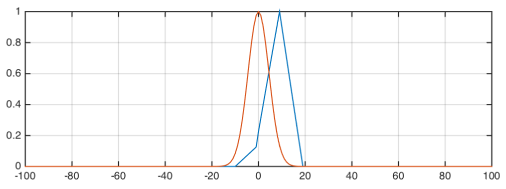
\includegraphics[width=\textwidth]{./Template_Figures/normal_ccr}
        \caption{}\label{fig:normal_ccr}
    \end{subfigure}

    \begin{subfigure}[b]{0.9\textwidth}
        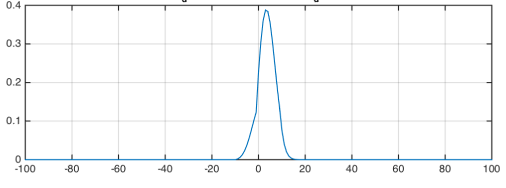
\includegraphics[width=\textwidth]{./Template_Figures/windowed_ccr}
        \caption{}\label{fig:windowed_ccr}
    \end{subfigure}

    \caption{(A) The scan line of the result of local cross-correlation of a cylinder with width and the disparity of 9 pixel (Blue). Red line represents a Gaussian with $\sigma$ = 9 pixels centered at the location of the ghost. (B) The resulting Gaussian weighed local cross-correlation. It can be seen that the disparity at the peek has shifted back.\label{fig:windowed_ccr_f}}
\end{figure}

In our disparity estimator model, we assume that the HVS will be able to isolate the object of interest in one source retinal image (due to luminance profile) and try to find an appropriate match for that object in the other i.e. target image. The target image consist of two possible matches i.e. the ghost and the object itself. For simplicity, we chose to compute the cross-correlation for a single scan-line of the stereo image pair. This would be sufficient to estimate the disparity of fixed width objects. Figure \ref{fig:normal_ccr} (blue) represents the cross-correlation profile for a cylinder that has a width of 9 pixels and is located at the disparity of 9 pixel. The background for simplicity in this case is black. We can see that there is some positive correlation at zero disparity due to the 14\% crosstalk ghost however, the full correlation (+1) is attained where the lag is 9 indicating the actual disparity of the object. The orange graph represents how the resulting correlation profile is weighted by a truncated Gaussian that has a standard deviation of 9 pixels. The Gaussian weighed correlation profile \ref{fig:windowed_ccr} is obtained by simple point-wise multiplication of the two functions in figure \ref{fig:normal_ccr}. It can be seen that after weighing with the Gaussian window for which the standard deviation $\sigma$ is roughly equal to the width of the object, the maximum correlation occurs at a lag of 3 pixels. Which shows that the perceived depth via disparity would be approximately 3 pixels (around 1.18 cm). So in this case the estimated disparity is quite close to the result that we obtained from the experiments.

\begin{figure}[H]
\centering
    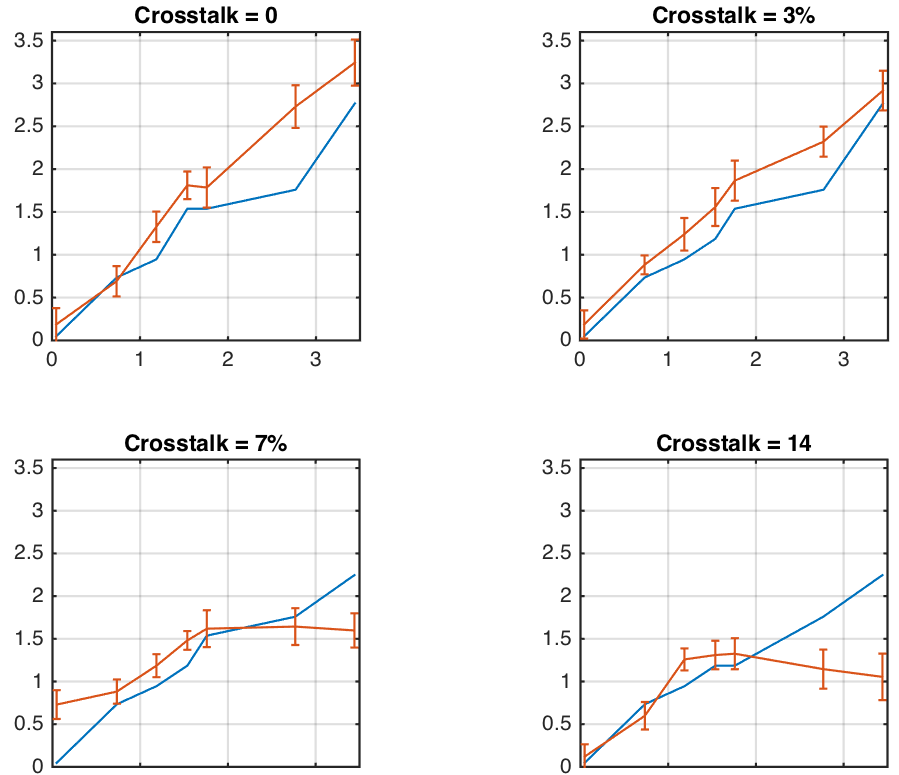
\includegraphics[width=0.7\textwidth]{./Template_Figures/s_9_sigma_7_4}
    \caption{Comparison of experimental observed depth for cylinder of 18.9 arc min width (orange) vs estimated depth via windowed cross-correlation. The best results were obtained with $\sigma$ = 15.4 arc min.\label{fig:s_9_sigma_7_4}}
\end{figure}
\begin{figure}[H]
\centering
    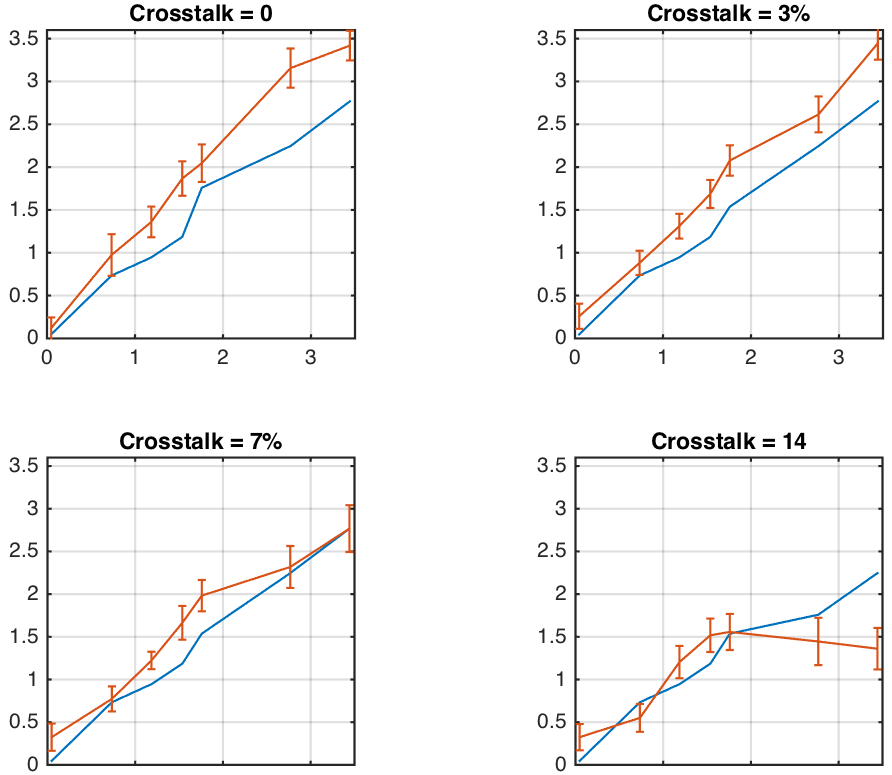
\includegraphics[width=0.7\textwidth]{./Template_Figures/s_18_sigma_14_7}
    \caption{Comparison of experimental observed depth for cylinder of 37.8 arc min width (orange) vs estimated depth via windowed cross-correlation. The best results were obtained with $\sigma$ = 30.87 arc min.\label{fig:s_18_sigma_14_7}}
\end{figure}
\begin{figure}[H]
\centering
    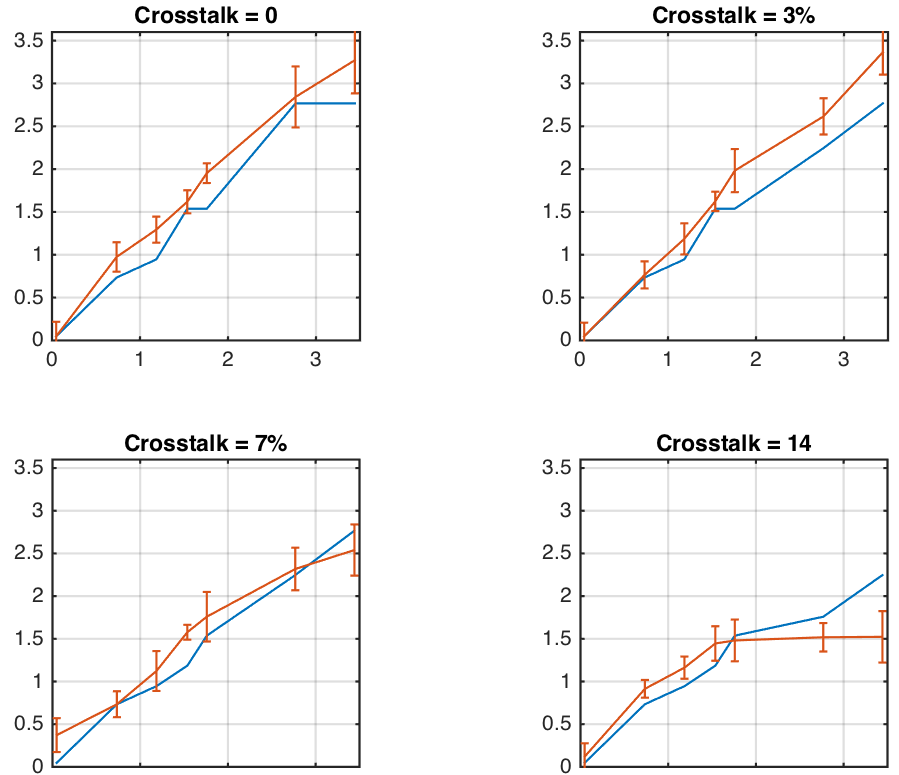
\includegraphics[width=0.7\textwidth]{./Template_Figures/s_27_sigma_17_4}
    \caption{Comparison of experimental observed depth for cylinder of 56.7 arc min width (orange) vs estimated depth via windowed cross-correlation. The best results were obtained with $\sigma$ = 36.54 arc min.\label{fig:s_27_sigma_17_4}}
\end{figure}
\begin{figure}[H]
\centering
    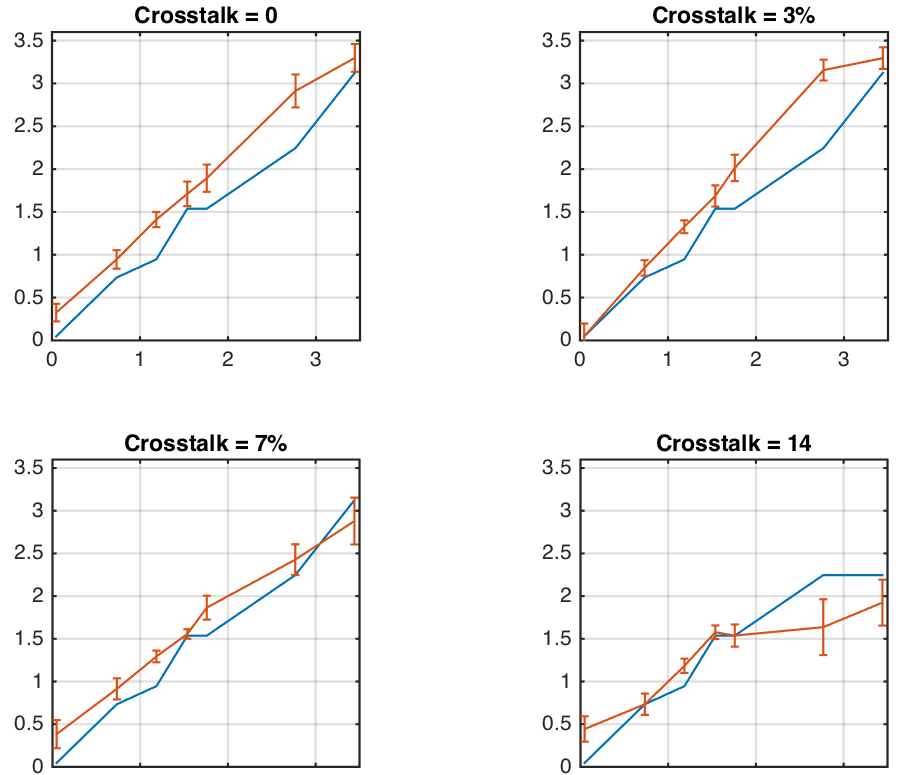
\includegraphics[width=0.7\textwidth]{./Template_Figures/s_36_sigma_22}
    \caption{Comparison of experimental observed depth for cylinder of 75.6 arc min width (orange) vs estimated depth via windowed cross-correlation. The best results were obtained with $\sigma$ = 46.2 arc min.\label{fig:s_36_sigma_22}}
\end{figure}

Next we simulated our stereo experiments for the cylinders and computed the estimated depth using our Gaussian weighted cross-correlation model. Figure \ref{fig:s_9_sigma_7_4} to Figure \ref{fig:s_36_sigma_22} shows the results that we obtained and there comparison with the data we got from our experiments. We observed that even thought this model had some short comings and did not fit to all of the data properly, it was able to mimic the degradation of estimated depth as the crosstalk level or the disparity increased. The figures above represents the estimated depth using a fixed $\sigma$ for each cylinder that best matched the data. For almost all the cases (specific disparities and crosstalk levels) where the estimated depth was incorrectly estimated, we were able get approximately matching results using some $\sigma$. But we were not able to find one $\sigma$ that matched all cases for a particular type of cylinder. Perhaps the HVS weighs the cross-correlation profile with Gaussians of different standard deviations for different object widths and disparities. Our Gaussian window weighted local cross-correlation model has an advantage that it resolves to a degraded estimates depth in case when certain level of crosstalk is present. However, the short coming is that it also penalizes the estimated depth to some level even if there is no crosstalk present. This does not conform very well to our experimental data but maybe it gives the right direction for the future research in this area.
\pagebreak

\section{Crosstalk mitigation}

During the course of this thesis, we devised and tested some new ideas that might be able to improve the current crosstalk reduction techniques. In the following section we review those ideas.

\subsection{Unsharp masking in epipolar domain}
Corn-sweet illusion \cite{ wiki:cornsweet} is used in contrast boosting image processing techniques such as unsharp masking. The basic idea of unsharp masking is to add to an image a high frequency image of itself. The high frequencies containing image is obtained by subtracting a blurred version of the image from itself. \cite{van2011perceptually} used similar technique to blur the uncorrectable crosstalk in combination with increasing the contrast of the object around the edges. One can generally use unsharp masking to subdue the perception of the uncorrectable ghosts. However applying unsharp masking in spatial domain also boosts the unwanted noise. Since automultiscopic screens displays lightfields, we thought that applying unsharp masking in the view domain (also called as the epipolar domain) would result in a crosstalk compensated lightfield with increased local contrast around the object. Let $\Psi$ be a lightfield in which x, y denote the spacial dimensions on the displayed image and w denotes the epipolar domain (Figure \ref{fig:lightfeild})
\begin{figure}[htbp]
\centering
    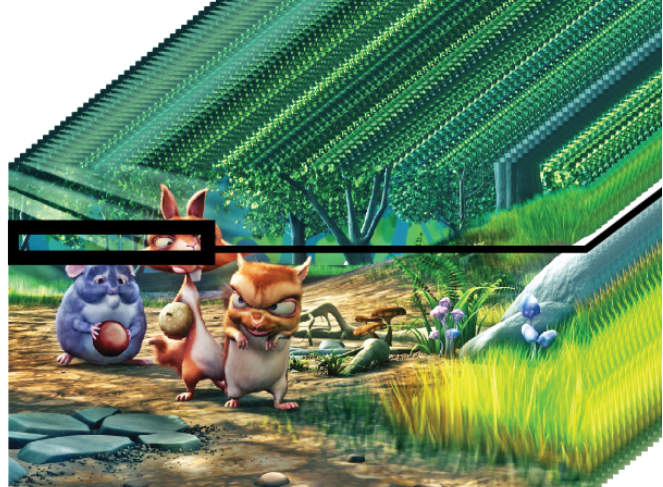
\includegraphics[width=0.7\textwidth]{./Template_Figures/lightfield}
    \caption{Representation of a 3D lightfield.\label{fig:lightfeild}}
\end{figure}
Then for an automultiscopic screen where only the light from the immediate neighbors is leaked, we blur the lightfield in epipolar domain with the following kernel. This will result in a epipolar domain blurred lightfield $\Psi_{blr}$
\begin{table}[htbp]
\centering
\begin{tabular}{|c|c|c|}
\hline
$\omega_1$ & $\omega_2$ & $\omega_3$ \\
\hline
\end{tabular}
\label{tab:blurring_kernel}
\end{table}

Next we subtract $\Psi_{blr}$ from the original Light Field $\Psi$. This will give us  $\Psi_{hf}$, a Light Field that only contains luminance-inverted ghosts in every view. i.e.
\begin{equation}
\Psi_{hf}\: =\: \Psi\: -\: \Psi_{blr}
\end{equation}
The crosstalk compensated lightfield is obtained as
\begin{equation}
\Psi_{opt}\: =\: \Psi\: +\: \Psi_{hf}
\end{equation}
Hence for every view image $I \in\: \Psi_{opt}$
\begin{equation}
\begin{aligned}
I_{opt}\: =\:  I + (I - \omega_1I_L - \omega_2I - \omega_3I_R) \\
I_{opt}\: = \: (2-\omega_2)\ I\: -\: \omega_1I_L\: -\: \omega_3I_R
\end{aligned}
\end{equation}
Where $I$ is the view centered image and $I_L, I_R$ are the immediate left and right neighbors. Since the automultiscopic screen will display the optimized Light Field image as a weighted sum of $I_L, I_R$ and $I$ i.e.
\begin{equation}
\begin{aligned}
I_{observed}\: =\:  \Phi_1.I_{L(opt)}\: + \:\Phi_2.I_{(opt)}\: + \:\Phi_3.I_{R(opt)}       \\
I_{observed}\: = \: \Phi_1{(2-\omega_2) I_L\: -\: \omega_1I_{LL}\: -\: \omega_3I}\:+  \\
                    \Phi_2{(2-\omega_2) I\: -\: \omega_1I_{L}\: -\: \omega_3I_R}\:+   \\
                    \Phi_3{(2-\omega_2) I_R\: -\: \omega_1I\: -\: \omega_3I_{RR}}
\end{aligned}
\end{equation}
Here $I_{LL}$ and $I_{RR}$ are the immediate left and right images to Left and right image of the view position in the lightfeild. We know from \ref{fig:sim_gaussians} that
\begin{equation}
\begin{aligned}
\Phi_1\:=\: \Phi_3\:=\: 0.0351,\:\: \Phi_2\:=\:0.8
\end{aligned}
\end{equation}
In order to cancel the effect of $I_L$ and $I_R$ we choose
\begin{equation}
\begin{aligned}
\omega_1\:=\: \omega_3\:=\: 0.0421,\:\: \omega_2\:=\:1.19
\end{aligned}
\end{equation}
The viewer observed image $I_{observed}$ can then be mathematically written as
\begin{equation}
I_{observed}\: =\:  1.42.I\:-\: 0.0014(I_{LL}\:+\:I_{RR})
\label{eq:final_unsharp_obs}
\end{equation}

It can be seen from equation \ref{eq:final_unsharp_obs} that even though the The crosstalk effect from the immediate left and right image of a view has been eliminated, some over-subtraction of luminance due to the $I_{LL}$ and $I_{RR}$ propagates in the observed image $I_{observed}$. Also, the average luminance of the view centered image $I$ has been increased to 1.42. Since the maximum luminance value an automultiscopic screen can display is 1, over proposed technique will result in clipping of the all the luminance values above 1 hence resulting in loss of contrast. More importantly, we described in figure \ref{fig:why_no_cornsweet}, it is impossible to obtain corn-sweet profiles by performing unsharp masking in view domain on a lightfeild.

\begin{figure}[htbp]
    \centering
    \begin{subfigure}[b]{0.48\textwidth}
        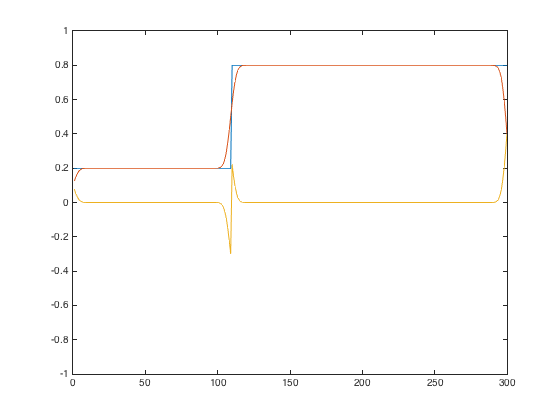
\includegraphics[width=\textwidth]{./Template_Figures/unsharp_proper}
        \caption{}\label{fig:cornsweet}
    \end{subfigure}
    \begin{subfigure}[b]{0.48\textwidth}
        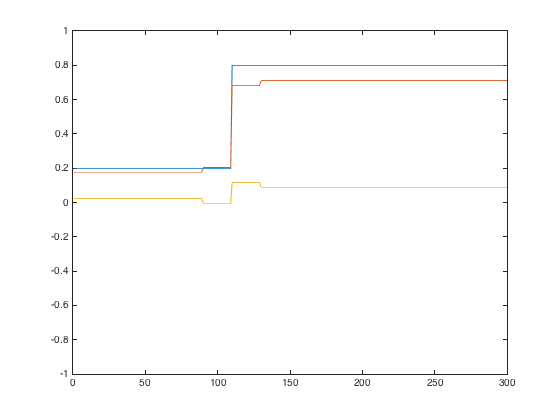
\includegraphics[width=\textwidth]{./Template_Figures/unsharp_epipolar}
        \caption{}\label{fig:no_cornsweet}
    \end{subfigure}

    \caption{(A) 1D representation of luminance profile along an image row. Blue graph represents a luminance step and orange graph represents the luminance profile of the blurred image. Yellow graph represents corn-sweet profile centered at the luminance edge and obtained as the difference between the original and the blurred image.  (B) Same procedure performed in view domain. Blue graph represents the luminance profile of a lightfeild image and orange graph represents the non-energy preserving additive blurring due to neighboring views in an automultiscopic environment. The Yellow graph represents the difference between the view image and its view-domain blurred version that resembles closely to subtractive crosstalk cancellation rather than a corn-sweet profile.\label{fig:why_no_cornsweet}}
\end{figure}

\subsection{Iterative crosstalk reduction}

To the best of our knowledge, all the current subtractive crosstalk reduction techniques compute the pre-processed crosstalk compensated images by subtracting the amount of leaked light between neighboring. The calculation of subtracted leaked light is always performed while considering the unmodified stereo image pair. We observe that the amount of light leaked into a view image due to the unmodified alternative view image should be different when the alternate view image is already crosstalk compensated. This is the case in reality and hence we think that a view image should be compensated appropriately if it alternative view image is already crosstalk compensated. Inspired by this idea, we propose an iterative subtractive crosstalk reduction technique.

Consider a lightfeild $\Psi$ consisting a set of view images ${f_1, f_2, ..., f_N}$. When the $i^{th}$ view is displayed on an automultiscopic screen, its crosstalk $\phi(f_i)$ from the neighboring views can be written as
\begin{equation}
\phi(f_i)\:=\: a_1.f_1\:+\:a_2.f_2\:+\:...\:a_{i-1}.f_{i-1}\:+\:a_{i+1}.f_{i+1}\:+\:...\:a_n.f_n
\end{equation}
Where the light intensity leakage values $a_1...a_n$ are chosen according to figure \ref{fig:sim_gaussians}. The crosstalk compensated images $\{\gamma_1...\gamma_n\}$ can then be computed iteratively as
\begin{equation}
\begin{aligned}
\gamma_1^{n+1} \:=\: f_1 \:+\: \phi(\gamma_1^n) \\
\gamma_2^{n+1} \:=\: f_2 \:+\: \phi(\gamma_2^n) \\
.\:\:\:\:\:\:\:\:\:\:\:\:\:\:\:\:\:\:\:\:\:\:\:\:\:\:\:\:\:\:\:\:\:\:\:\:\:\ \\
.\:\:\:\:\:\:\:\:\:\:\:\:\:\:\:\:\:\:\:\:\:\:\:\:\:\:\:\:\:\:\:\:\:\:\:\:\:\ \\
.\:\:\:\:\:\:\:\:\:\:\:\:\:\:\:\:\:\:\:\:\:\:\:\:\:\:\:\:\:\:\:\:\:\:\:\:\:\ \\
\gamma_N^{n+1} \:=\: f_N \:+\: \phi(\gamma_N^n) \\
\end{aligned}
\end{equation}
Where `n' is the number of current iteration. After each iteration, clipping of the values exceeding the display's dynamic range is performed. The iterations terminate when an error $\epsilon$ falls below a threshold.
\begin{equation}
\begin{aligned}
\epsilon \:=\: \sqrt{(\gamma_1^{n+1}\:-\:\gamma_1^n)^2 \:+\: ...\:+\:(\gamma_N^{n+1}\:-\:\gamma_N^n)^2}
\end{aligned}
\end{equation}

This technique compensates for the crosstalk more appropriately however, the successive subtraction of luminance from the lightfeild view images between iterations might result in lower average luminance in the crosstalk compensated lightfeild (figure \ref{fig:iterative_tech}
\begin{figure}[htbp]
    \centering
    \begin{subfigure}[b]{0.48\textwidth}
        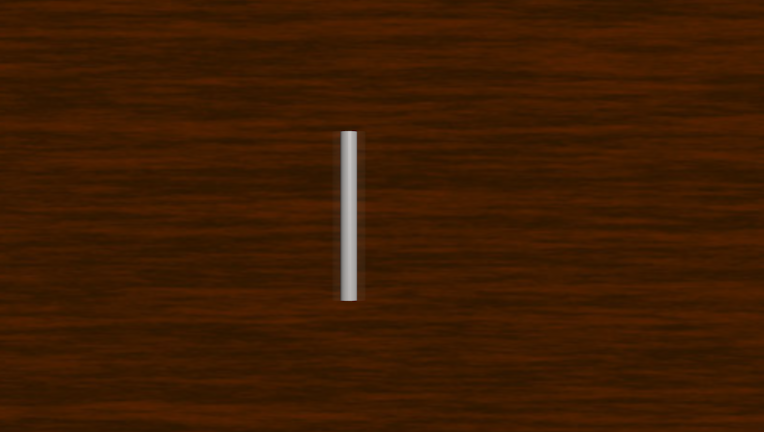
\includegraphics[width=\textwidth]{./Template_Figures/image_w_ct}
        \caption{}\label{fig:original_lf}
    \end{subfigure}

    \begin{subfigure}[b]{0.48\textwidth}
        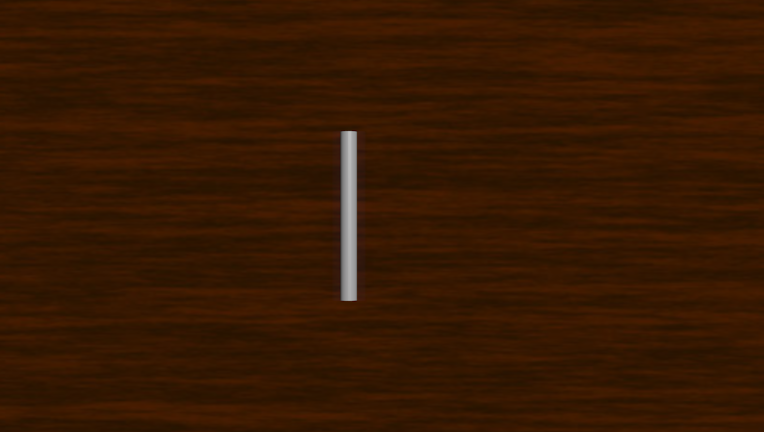
\includegraphics[width=\textwidth]{./Template_Figures/subtractive_comp}
        \caption{}\label{fig:subtractive_lf}
    \end{subfigure}
    \begin{subfigure}[b]{0.48\textwidth}
        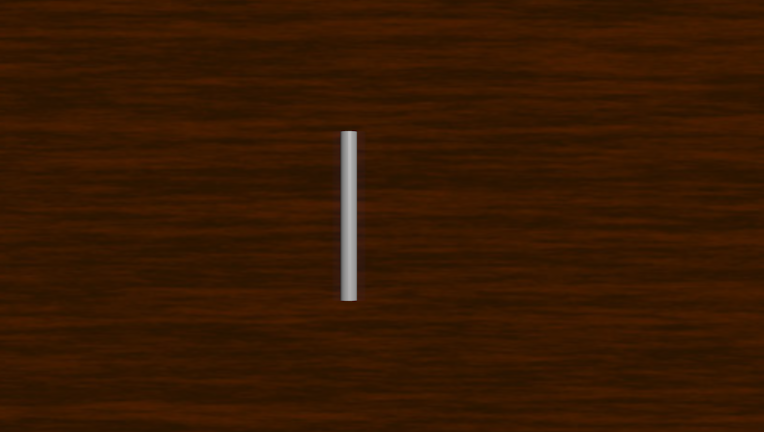
\includegraphics[width=\textwidth]{./Template_Figures/iterative_comp}
        \caption{}\label{fig:iterative_lf}
    \end{subfigure}

    \caption{(A) \label{fig:iterative_tech}}
\end{figure}


% \subsection{Proposed optimizations}
% \subsection{Unsharp masking in view domain}
% \subsection{Iterative subtraction}
